\documentclass[11pt,a4paper]{article}

\usepackage[utf8]{inputenc}
\usepackage[T1]{fontenc}
\usepackage{lmodern}
\usepackage{microtype}
\usepackage{geometry}
\geometry{left=2.4cm,right=2.4cm,top=2.5cm,bottom=2.5cm}
\usepackage{enumitem}
\usepackage{hyperref}
\usepackage{amsmath}
\usepackage{amssymb}
\usepackage{booktabs}
\usepackage{tabularx}
\usepackage{array}
\usepackage{makecell}
\usepackage{float}
\usepackage{caption}
\usepackage{xcolor}
\usepackage{tikz}
\usetikzlibrary{arrows.meta,positioning,calc,shapes.geometric}
\usepackage{pgfplots}
\pgfplotsset{compat=1.18}

\definecolor{ink}{HTML}{20262E}
\definecolor{bluebase}{HTML}{3B6EA8}
\definecolor{goldbase}{HTML}{C28B2C}
\definecolor{tealbase}{HTML}{3B8178}
\definecolor{quiet}{HTML}{69727D}
\definecolor{grid}{HTML}{D9DEE3}
\definecolor{panel}{HTML}{F4F6F8}

\hypersetup{
  colorlinks=true,
  linkcolor=bluebase!75!black,
  urlcolor=bluebase!75!black,
  citecolor=bluebase!75!black,
  pdftitle={Expiry-Aware Successor Selection: Technical Methodology and Results}
}

\setlist[itemize]{topsep=3pt,itemsep=2pt,parsep=0pt}
\setlist[enumerate]{topsep=3pt,itemsep=2pt,parsep=0pt}
\renewcommand{\arraystretch}{1.2}
\newcommand{\code}[1]{\texttt{\small #1}}
\newcommand{\pathcode}[1]{{\small\nolinkurl{#1}}}
\newcommand{\method}{\code{M\_E\_expiry\_aware\_text}}

\tikzset{
  stage/.style={
    rectangle,rounded corners=3pt,draw=quiet!75,fill=panel,
    minimum height=0.95cm,text width=3.25cm,align=center,
    font=\small\sffamily,inner sep=5pt
  },
  oldstage/.style={stage,draw=bluebase!85!black,fill=bluebase!9},
  newstage/.style={stage,draw=goldbase!90!black,fill=goldbase!10},
  outstage/.style={stage,draw=tealbase!90!black,fill=tealbase!9},
  flow/.style={-Stealth,thick,draw=quiet!85}
}

\title{%
  {\Large\bfseries Expiry-Aware Successor Selection}\\[5pt]
  {\large Technical Methodology and Results}\\[3pt]
  {\normalsize BOAMP Grand Ouest Digital Procurement Pipeline}
}
\author{BOAMP Data Science Internship Project}
\date{12 August 2026}

\begin{document}

\maketitle

\begin{abstract}
This report documents the implemented expiry-aware successor-selection policy for
the BOAMP Grand Ouest digital procurement study. The policy leaves broad candidate
generation unchanged and modifies only candidate selection. A candidate published
more than one year before the best observable expected contract end must satisfy
stronger text and CPV continuity requirements. Applied to 3,800 cohort contracts and
868,527 candidate pairs, the policy accepts 507 observable successor procurements,
compared with 547 under the frozen text-only baseline. Reviewed-benchmark metrics are
unchanged: precision 0.8000, recall 0.3636, and zero false positives on reviewed
negative anchors. The automatic promotion gate passes, but the method remains a
parallel sensitivity arm until 42 changed links receive manual review. Accepted links
are observable successor procurements, not confirmed legal renewals.

The underlying modeling phase is implemented, not proposed. Four pre-existing
linkage methods were fitted or executed and compared before the expiry-aware fifth
policy was added. This report includes their algorithms, operating points, benchmark
results, and failure analysis so that implementation status can be audited directly.
\end{abstract}

\tableofcontents
\clearpage

\section{Technical Summary}

The expiry-aware policy is more conservative and more explicitly aligned with contract
timing than the frozen baseline because it addresses a documented failure mode: a
public buyer can publish many unrelated
procurements while an existing contract is active. The baseline
\code{M\_B\_text\_ranking} method accepts a same-buyer candidate primarily from text
similarity, so repeated buyer and administrative language can produce an implausibly
early link. The new policy retains broad retrieval but raises the evidence standard
for candidates more than 365 days before expected expiry.

The implemented result is conservative:

\begin{itemize}
  \item candidate generation remains fixed at 868,527 pairs;
  \item accepted links fall from 547 to 507;
  \item 505 baseline pairs are retained, 42 are removed, and 2 replacement pairs are selected;
  \item the survival event rate falls from 14.39\% to 13.34\%;
  \item median observed time to successor rises from 32.07 to 34.40 months;
  \item all four digital segments retain more than 30 observed events;
  \item benchmark precision, recall, and false-positive rate are unchanged.
\end{itemize}

The new method passes the pre-specified numerical promotion gate. This is not
sufficient for automatic promotion: expiry is unavailable for 2,845 of 3,800
contracts, and the small benchmark does not independently validate most changed
links. The operational decision is to keep the method parallel until the complete
42-row review queue is adjudicated.

\section{Implemented Boundary and Data Scope}

\subsection{The change occurs after candidate generation}

Figure~\ref{fig:pipeline} locates the new step within the implemented pipeline. Raw
acquisition, standardisation, episode reconstruction, cohort definition, same-buyer
blocking, and the broad temporal window are unchanged. The policy enriches existing
candidate pairs with expiry evidence and applies an additional acceptance rule.

\begin{figure}[H]
\centering
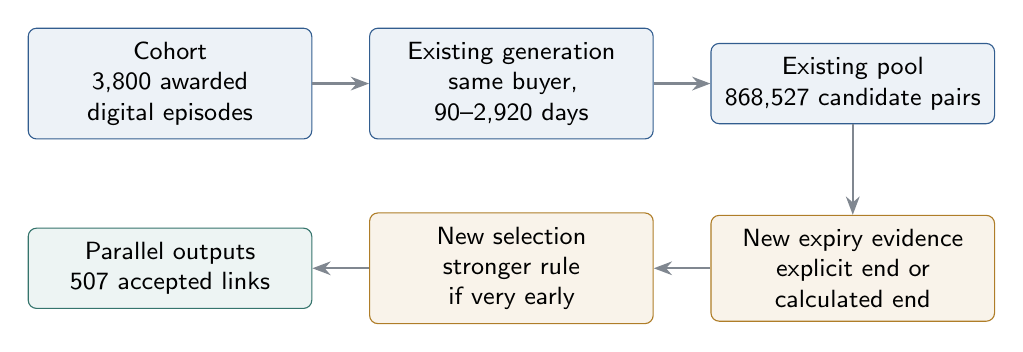
\begin{tikzpicture}[node distance=0.72cm]
  \node[oldstage] (cohort) {Cohort\\3,800 awarded digital episodes};
  \node[oldstage,right=0.72cm of cohort] (generation) {Existing generation\\same buyer, 90--2,920 days};
  \node[oldstage,right=0.72cm of generation] (pool) {Existing pool\\868,527 candidate pairs};
  \node[newstage,below=1.15cm of pool] (expiry) {New expiry evidence\\explicit end or calculated end};
  \node[newstage,left=0.72cm of expiry] (selection) {New selection\\stronger rule if very early};
  \node[outstage,left=0.72cm of selection] (outputs) {Parallel outputs\\507 accepted links};
  \draw[flow] (cohort) -- (generation);
  \draw[flow] (generation) -- (pool);
  \draw[flow] (pool) -- (expiry);
  \draw[flow] (expiry) -- (selection);
  \draw[flow] (selection) -- (outputs);
\end{tikzpicture}
\caption{Pipeline boundary of the expiry-aware method. Blue stages are unchanged;
gold stages are new; the green stage contains parallel v2 outputs.}
\label{fig:pipeline}
\end{figure}

\subsection{Population, grain, and observation period}

The study cohort contains 3,800 procurement episodes. Each episode is a Grand Ouest
public procurement with at least one digital CPV division in
$\{32,35,48,72\}$ and an award notice. One cohort row represents one awarded
procurement episode. The award-notice publication date is time zero. The corpus and
right-censoring cutoff end on 31 December 2025.

The candidate pool contains one row per ordered anchor--candidate episode pair. A
candidate must belong to the same buyer block and be published between 90 and 2,920
days after the anchor award. Candidate episodes are not restricted to digital CPVs
or award notices because a successor can first appear as a tender and may be
incompletely coded.

\section{Notation and Metric Definitions}

Table~\ref{tab:notation} defines each symbol before it is used in the model
specification.

\begin{table}[H]
\centering
\caption{Notation for expiry-aware successor selection.}
\label{tab:notation}
\small
\begin{tabularx}{\textwidth}{p{2.6cm}X}
\toprule
\textbf{Symbol} & \textbf{Definition} \\
\midrule
$a$ & Anchor contract in the 3,800-row survival cohort. \\
$c$ & Later candidate procurement episode from the same buyer block. \\
$A_a$ & Award-notice publication date of anchor $a$. \\
$C_c$ & First-notice publication date of candidate $c$. \\
$D_a$ & Reliable declared duration of anchor $a$, measured in months. \\
$S_a$ & Unambiguous explicit contract start date, when observable. \\
$F_a$ & Unambiguous explicit contract end date, when valid and observable. \\
$E_a$ & Best available expected end date of anchor $a$. \\
$R_{ac}$ & Candidate timing relative to expected end, $C_c-E_a$, in days. \\
$s_t(a,c)$ & Maximum word- or character-TF--IDF cosine similarity in $[0,1]$. \\
$s_k(a,c)$ & CPV continuity score; positive values indicate shared CPV hierarchy. \\
$S(a,c)$ & Existing weighted linkage score in $[0,100]$, used as a tie-breaker. \\
$m_j(\ell)$ & Probability of comparison level $\ell$ for field $j$ among matches. \\
$u_j(\ell)$ & Probability of comparison level $\ell$ for field $j$ among non-matches. \\
$\lambda$ & Fellegi--Sunter prior probability that a candidate pair is a match. \\
$M(a,c)$ & Fellegi--Sunter log$_2$ match weight for pair $(a,c)$. \\
$\widehat{y}_a$ & Selected observable successor for $a$, or $\varnothing$ if the method abstains. \\
$\delta_a$ & Survival event indicator: 1 if a successor is selected, otherwise 0. \\
$T_a$ & Observed time from award to successor, or award to cutoff when censored. \\
\bottomrule
\end{tabularx}
\end{table}

Let TP be a selected candidate that equals a reviewed successor, FP a selected wrong
candidate or a selection on a reviewed no-successor anchor, and FN a reviewed
successor not selected at rank one. Then

\begin{equation}
  \operatorname{Precision@1}=\frac{\mathrm{TP}}{\mathrm{TP}+\mathrm{FP}},
  \qquad
  \operatorname{Recall@1}=\frac{\mathrm{TP}}{\mathrm{TP}+\mathrm{FN}}.
\end{equation}

The reported false-positive rate is defined on reviewed negative anchors:

\begin{equation}
  \operatorname{FPR}_{-}=\frac{\text{negative anchors receiving a link}}
  {\text{reviewed negative anchors}}.
\end{equation}

\section{Candidate Evidence and Implemented Algorithms}

\subsection{The model phase is materialised and executable}

Table~\ref{tab:implementation} separates implemented code and outputs from future
work. Every row shown as implemented has an executable script, a materialised
artifact, and automated validation or benchmark evidence.

\begin{table}[H]
\centering
\caption{Implementation audit of the linkage-model phase.}
\label{tab:implementation}
\small
\begin{tabularx}{\textwidth}{p{3.2cm}p{2.0cm}X}
\toprule
\textbf{Component} & \textbf{State} & \textbf{Material evidence} \\
\midrule
Candidate features & Implemented & 868,527 rows in
\pathcode{linkage_candidates.parquet}. \\
Deterministic method $M_A$ & Implemented & Executed by
\pathcode{scripts/evaluate_linkage.py}. \\
Text-ranking method $M_B$ & Implemented & Frozen v1 operating point at 0.70. \\
Weighted gated method $M_C$ & Implemented & Executed at score threshold 70 and
retained as a high-recall sensitivity arm. \\
Fellegi--Sunter $M_D$ & Fitted & EM model in
\pathcode{fellegi_sunter_model.json}; scored values for every candidate pair. \\
Expiry-aware method $M_E$ & Implemented & 507 accepted links plus the 42-anchor
review artifact. \\
Threshold evaluation & Implemented & Pilot grid and all-method comparison CSVs. \\
Survival conversion & Implemented & Parallel 3,800-row dataset with structural
validation. \\
\bottomrule
\end{tabularx}
\end{table}

\subsection{Four interpretable evidence components are computed}

All methods operate on the same candidate pairs, but they use the evidence
components differently.

\paragraph{Buyer evidence.}
Buyer matching distinguishes a validated SIREN match, an exact normalised-name
match, fuzzy-name evidence, token overlap, and no match. The score mapping is

\begin{equation}
s_b(a,c) \in \{1.00,0.90,0.70,0.60,0.00\},
\end{equation}

in that order. Candidate blocking already requires the same exact buyer key or
normalised blocking name; this score measures the strength of that identity evidence.
Simple raw case variants such as \code{Ville de Paris} and \code{VILLE DE PARIS}
normalise to the same name. Organisational suffixes remain distinct unless a shared
validated SIREN or the blocking-name rule provides continuity; this is formatting
normalisation, not complete buyer entity resolution.

\paragraph{Text evidence.}
Text is normalised to lowercase accent-free alphanumeric tokens. For each anchor
block, separate word TF--IDF vectors with 1--2 grams and character TF--IDF vectors
with 3--5 character grams are fitted. Let $\mathbf{x}^{(w)}$ and
$\mathbf{x}^{(q)}$ denote word and character vectors. The implemented text score is

\begin{equation}
s_t(a,c)=\max\left\{
\frac{\mathbf{x}^{(w)}_a\cdot\mathbf{x}^{(w)}_c}
{\lVert\mathbf{x}^{(w)}_a\rVert\lVert\mathbf{x}^{(w)}_c\rVert},
\frac{\mathbf{x}^{(q)}_a\cdot\mathbf{x}^{(q)}_c}
{\lVert\mathbf{x}^{(q)}_a\rVert\lVert\mathbf{x}^{(q)}_c\rVert}
\right\}.
\end{equation}

Local fitting makes common boilerplate within one buyer less influential than rare
terms describing the repeated purchasing need. Character grams preserve evidence
when spelling, accents, abbreviations, or word boundaries vary.

\paragraph{CPV continuity.}
Let $G_3(e)$ be the set of three-digit CPV groups in episode $e$, $G_2(e)$ its
two-digit divisions, and $J(X,Y)=|X\cap Y|/|X\cup Y|$ the Jaccard coefficient. Then

\begin{equation}
s_k(a,c)=\max\left\{J(G_3(a),G_3(c)),\;0.5J(G_2(a),G_2(c))\right\}.
\end{equation}

The score is missing, not zero, if either episode has no CPV. A zero means that both
sides are coded and disagree; missing means continuity is unobservable.

\paragraph{Timing plausibility.}
Let $g_{ac}=C_c-A_a$ be the award-to-candidate gap and let
$d_a=30.4375D_a$ be expected duration in days. Where duration is reliable,

\begin{equation}
s_{\tau}(a,c)=\max\left\{0,1-\frac{|g_{ac}-d_a|}{365}\right\}.
\end{equation}

The score is missing when duration is unresolved or conflicting. The implementation
does not substitute a four-year default.

\paragraph{Weighted score.}
Let $\mathcal{O}(a,c)$ be the observable component set. The implemented weights are
shown in buyer, text, CPV, and timing order:

\begin{equation}
(w_b,w_t,w_k,w_{\tau})=(0.50,0.25,0.20,0.05).
\end{equation}

The combined score is

\begin{equation}
S(a,c)=100\,
\frac{\sum_{j\in\mathcal{O}(a,c)}w_js_j(a,c)}
{\sum_{j\in\mathcal{O}(a,c)}w_j}.
\label{eq:weightedscore}
\end{equation}

Renormalisation prevents missing evidence from acting like disagreement. It can also
make a score rely on fewer dimensions, which is why $M_C$ adds independent gates.

\subsection{Five linkage methods have defined algorithms}

\paragraph{$M_A$: deterministic SIREN--CPV rule.}
The candidate is eligible only when the buyer has the same validated SIREN,
$s_k(a,c)>0$, and $s_t(a,c)\ge0.25$. Eligible candidates are ranked by the weighted
score. This tests what rigid structured identity and category continuity can achieve.

\paragraph{$M_B$: same-buyer text ranking.}
Within the already blocked same-buyer pool,

\begin{equation}
I_B(a,c)=\mathbf{1}[s_t(a,c)\ge\theta_B].
\end{equation}

The frozen operating point is $\theta_B=0.70$, and eligible candidates are ranked by
$s_t$. This is the v1 baseline because it achieved the strongest reviewed precision
and zero false positives on reviewed negative anchors.

\paragraph{$M_C$: weighted score with independent gates.}
At the evaluated operating point, $M_C$ requires all of the following:

\begin{itemize}
  \item strong buyer evidence: SIREN, exact normalised name, or fuzzy-name similarity
  at least 0.82;
  \item $s_t\ge0.25$;
  \item positive CPV continuity, or $s_t\ge0.55$ as a text override;
  \item if buyer evidence is weaker than SIREN or exact name, $s_t\ge0.40$ and
  positive CPV continuity;
  \item weighted score $S(a,c)\ge70$.
\end{itemize}

Eligible candidates are ranked by $S(a,c)$. The method is designed to recover more
successors while requiring evidence from several dimensions.

\paragraph{$M_D$: unsupervised Fellegi--Sunter model.}
Buyer, text, CPV, and timing comparisons are discretised into levels. For field $j$
and observed level $\ell_j$, the model estimates

\begin{equation}
m_j(\ell_j)=P(\ell_j\mid\text{match}),\qquad
u_j(\ell_j)=P(\ell_j\mid\text{non-match}).
\end{equation}

Assuming conditional independence, evidence is accumulated as a log Bayes factor:

\begin{equation}
M(a,c)=\log_2\frac{\lambda}{1-\lambda}
+\sum_j\log_2\frac{m_j(\ell_j)}{u_j(\ell_j)},
\end{equation}

with posterior

\begin{equation}
P(\text{match}\mid a,c)=\frac{2^{M(a,c)}}{1+2^{M(a,c)}}.
\end{equation}

Expectation maximisation alternates between pair-level match responsibilities and
updated $m$ distributions and $\lambda$. The primary fit fixes $u$ to population
comparison frequencies, uses Laplace smoothing 0.5, converges monotonically in 98
iterations, and scores every candidate pair. A free-$u$ fit is retained as a
robustness check. Candidates are accepted by a posterior threshold and ranked by the
posterior; the comparison point is 0.65.

\paragraph{$M_E$: expiry-aware text ranking.}
The fifth method is the v2 policy specified in Section~\ref{sec:expiry-method}. It
retains the $M_B$ rule except that a candidate more than 365 days before expected end
requires $s_t\ge0.85$ and $s_k>0$. It is a fixed rule, not a retrained model.

\section{Model Evaluation and Selection}

\subsection{The benchmark and retrieval stage are both evaluated}

The reference data were remapped to v2 episode IDs through stable BOAMP notice IDs.
Of 92 benchmark anchors, 85 are evaluable in the cohort: 22 positives and 63 reviewed
no-successor anchors. The pilot-development split has 16 anchors, including only 5
positives; the already-inspected locked split has 69 anchors, including 17 positives.

Before method-specific acceptance, candidate retrieval places the true successor at
rank one for 72.73\% of positive anchors, within rank five for 86.36\%, within rank
ten for 86.36\%, and within rank twenty for 90.91\%. Twenty-one of 22 reviewed
successors occur somewhere in the pool; the worst retrieved rank is 27. Thus the
acceptance methods cannot recover one positive that candidate generation does not
retrieve.

\subsection{Thresholds were evaluated, not supervised-fitted}

$M_A$, $M_B$, and $M_C$ were evaluated over thresholds
$\{50,55,60,65,70,75,80\}$. $M_D$ used posterior thresholds
$\{20,30,40,50,55,60,65,70\}$. These are operating-point comparisons, not
supervised model fine-tuning. With only five pilot positives, one changed prediction
moves pilot recall by 0.20, so the frozen choice was documented judgement rather than
an automatic maximum over noisy pilot metrics.

\subsection{All five methods are compared at their implemented operating points}

\begin{table}[H]
\centering
\caption{All-method benchmark comparison on 85 evaluable anchors.}
\label{tab:allmethods}
\small
\begin{tabular}{lrrrrr}
\toprule
\textbf{Method} & \textbf{Threshold} & \textbf{Precision} & \textbf{Recall@1} &
\textbf{FPR$_-$} & \textbf{Coverage} \\
\midrule
$M_A$ deterministic & rule & 0.5556 & 0.4545 & 0.1270 & 0.2118 \\
$M_B$ text ranking & 0.70 & \textbf{0.8000} & 0.3636 & \textbf{0.0000} & 0.1176 \\
$M_C$ weighted gated & 70 & 0.5714 & \textbf{0.7273} & 0.1587 & 0.3294 \\
$M_D$ Fellegi--Sunter & 0.65 & 0.3750 & 0.2727 & 0.0952 & 0.1882 \\
$M_E$ expiry-aware & 0.70 / 0.85 & \textbf{0.8000} & 0.3636 & \textbf{0.0000} & 0.1176 \\
\bottomrule
\end{tabular}
\end{table}

Figure~\ref{fig:methodcomparison} makes the precision--recall trade-off visible.
$M_B$ and $M_E$ prioritise precision and abstention; $M_C$ prioritises recall at the
cost of substantially more false positives.

\begin{figure}[H]
\centering
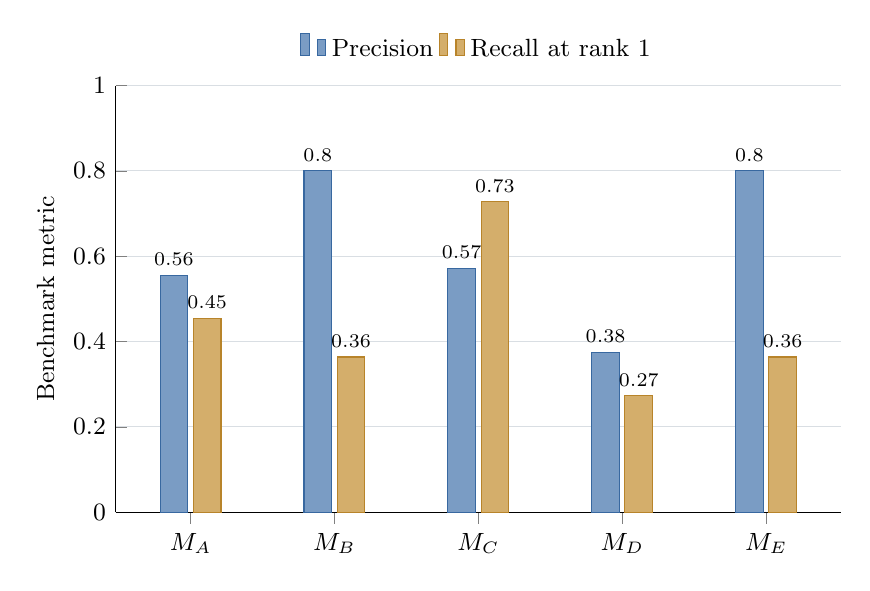
\begin{tikzpicture}
\begin{axis}[
  ybar,width=0.89\textwidth,height=7.0cm,ymin=0,ymax=1.0,
  symbolic x coords={$M_A$,$M_B$,$M_C$,$M_D$,$M_E$},xtick=data,
  ylabel={Benchmark metric},bar width=10pt,enlarge x limits=0.13,
  ymajorgrids=true,grid style={draw=grid},axis x line*=bottom,axis y line*=left,
  tick label style={font=\small},label style={font=\small},
  legend style={at={(0.5,1.03)},anchor=south,legend columns=2,draw=none,font=\small},
  nodes near coords,nodes near coords align={vertical},
  every node near coord/.append style={font=\scriptsize,/pgf/number format/.cd,fixed,precision=2}
]
\addplot[fill=bluebase!68,draw=bluebase!95!black] coordinates {
  ($M_A$,0.5556) ($M_B$,0.8000) ($M_C$,0.5714) ($M_D$,0.3750) ($M_E$,0.8000)
};
\addplot[fill=goldbase!70,draw=goldbase!95!black] coordinates {
  ($M_A$,0.4545) ($M_B$,0.3636) ($M_C$,0.7273) ($M_D$,0.2727) ($M_E$,0.3636)
};
\legend{Precision,Recall at rank 1}
\end{axis}
\end{tikzpicture}
\caption{Precision and rank-one recall by implemented method on all evaluable
benchmark anchors. The equal $M_B$ and $M_E$ bars mean the expiry rule does not alter
the small benchmark, not that the two policies are identical on the full cohort.}
\label{fig:methodcomparison}
\end{figure}

\subsection{Why each method works or fails}

\begin{itemize}
  \item \textbf{$M_A$ is rigid but not sufficiently precise.} Validated buyer identity
  and broad CPV continuity still occur across unrelated procurements from active
  buyers. It misses links without SIREN or CPV evidence and still links 8 of 63
  reviewed negative anchors.
  \item \textbf{$M_B$ succeeds through repeated need-specific language.} Same-buyer
  blocking removes the hardest identity problem, while high local TF--IDF similarity
  captures repeated procurement subjects. Its 0.70 floor gives the best reviewed
  precision and zero negative-anchor FPR, but abstention limits recall to 0.3636.
  \item \textbf{$M_C$ recovers positives but over-links.} It reaches recall 0.7273,
  but accepts 10 of 63 reviewed negative anchors. Buyer evidence is common by design
  after blocking, broad CPV continuity is not unique to one contract, and score
  renormalisation can leave fewer observed dimensions. It remains useful only as a
  high-recall sensitivity arm.
  \item \textbf{$M_D$ converges numerically but is not calibrated.} The primary EM fit
  estimates $\lambda=0.05267$, far above the real successor-pair rarity, while the
  free-$u$ robustness fit reaches the 0.5 guardrail. No posterior exceeds 0.90. The
  model learns dominant text and documentation structures rather than the extremely
  rare successor class; conditional dependence between fields also violates its
  simplifying assumption. It achieves precision 0.3750 and is not adopted.
  \item \textbf{$M_E$ targets a full-cohort error pattern absent from the benchmark.}
  It preserves $M_B$ metrics while changing 42 anchors in the complete application.
  This supports non-degradation, but manual review is required to establish whether
  those changes improve real precision.
\end{itemize}

\section{Expiry-Aware Selection Method}
\label{sec:expiry-method}

\subsection{Broad temporal retrieval remains unchanged}

The candidate-generation interval is intentionally broad. A pair $(a,c)$ is
temporally eligible for the existing pool when

\begin{equation}
  A_a+90\ \text{days} \le C_c \le A_a+2920\ \text{days}.
  \label{eq:broadwindow}
\end{equation}

Equation~\ref{eq:broadwindow} is a retrieval window, not an expiry window. It avoids
missing early re-tenders, delayed replacements, or successors whose contract dates
are unavailable. Expiry evidence is applied during selection rather than blocking.

\subsection{Expected end follows a fixed evidence hierarchy}

The best available expected end is resolved as

\begin{equation}
E_a =
\begin{cases}
F_a, & \text{if exactly one valid explicit end date exists},\\
S_a + D_a, & \text{if one start date and reliable duration exist},\\
A_a + D_a, & \text{if reliable duration exists},\\
\text{missing}, & \text{otherwise}.
\end{cases}
\label{eq:enddate}
\end{equation}

An explicit end is valid only when it is later than the award-notice date. Multiple
distinct start or end dates are not averaged. A duration is used only when episode
reconstruction reports \code{typed\_consensus}. Missing duration is not replaced by
a four-year assumption or any other default.

\begin{figure}[H]
\centering
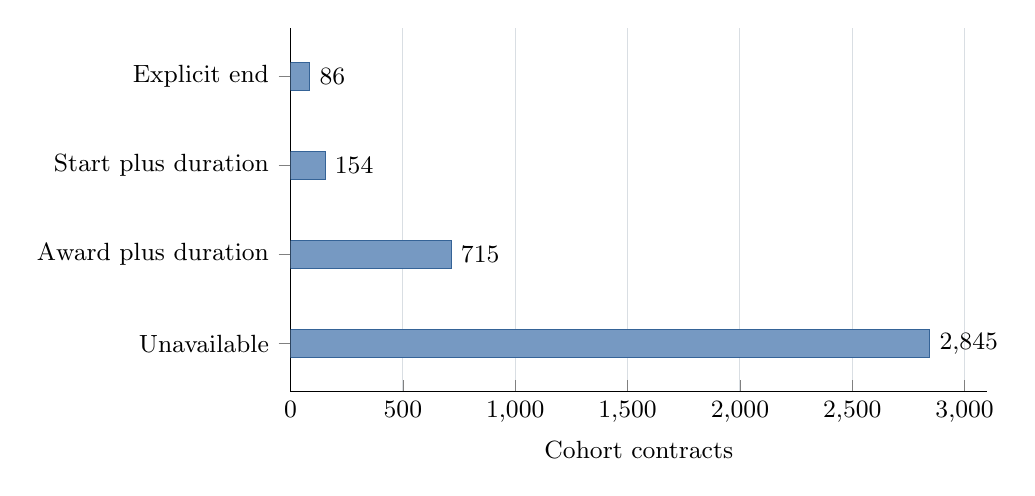
\begin{tikzpicture}
\begin{axis}[
  xbar,width=0.86\textwidth,height=6.2cm,xmin=0,xmax=3100,
  symbolic y coords={Explicit end,Start plus duration,Award plus duration,Unavailable},
  ytick=data,y dir=reverse,xlabel={Cohort contracts},
  xtick={0,500,1000,1500,2000,2500,3000},
  axis x line*=bottom,axis y line*=left,xmajorgrids=true,grid style={draw=grid},
  tick label style={font=\small},label style={font=\small},nodes near coords,
  every node near coord/.append style={font=\small,anchor=west},enlarge y limits=0.18
]
\addplot[fill=bluebase!70,draw=bluebase!90!black] coordinates {
  (86,Explicit end) (154,Start plus duration)
  (715,Award plus duration) (2845,Unavailable)
};
\end{axis}
\end{tikzpicture}
\caption{Expected-end evidence among 3,800 cohort contracts. Only 955 contracts
(25.1\%) receive a resolved expected end; unavailable expiry preserves the baseline
text threshold.}
\label{fig:expirysources}
\end{figure}

\subsection{Timing is measured relative to expected end}

For every candidate with a resolved anchor expiry,

\begin{equation}
  R_{ac}=C_c-E_a.
  \label{eq:relative}
\end{equation}

Negative $R_{ac}$ means the candidate was published before expected expiry. The
implemented classes are:

\begin{equation}
\operatorname{class}(a,c)=
\begin{cases}
\texttt{expiry\_unknown}, & E_a\text{ is missing},\\
\texttt{early\_more\_than\_1y}, & R_{ac}<-365,\\
\texttt{pre\_expiry\_within\_1y}, & -365\le R_{ac}<0,\\
\texttt{post\_expiry\_within\_1y}, & 0\le R_{ac}\le365,\\
\texttt{post\_expiry\_more\_than\_1y}, & R_{ac}>365.
\end{cases}
\end{equation}

The boundary is exact: a candidate published exactly 365 days before expected expiry
uses the normal rule. Only candidates earlier than that boundary receive the stronger
gate.

\subsection{Very early candidates require stronger functional evidence}

Define the eligibility indicator $I_{ac}$ as

\begin{equation}
I_{ac}=
\begin{cases}
\mathbf{1}\!\left[s_t(a,c)\ge0.85\ \land\ s_k(a,c)>0\right],
  & R_{ac}<-365,\\
\mathbf{1}\!\left[s_t(a,c)\ge0.70\right],
  & \text{otherwise}.
\end{cases}
\label{eq:eligibility}
\end{equation}

The second branch includes missing expiry. Missing CPV cannot pass the unusually
early branch because missing evidence is not positive continuity. Among eligible
candidates, ranking is deterministic: descending text similarity, descending
existing linkage score, ascending candidate origin date, then ascending candidate
episode identifier. One top candidate is selected per anchor, or the method abstains.
This is a fixed policy, not a newly fitted model.

\section{Results: Fewer Implausibly Early Events Without Benchmark Loss}

\subsection{The policy changes 42 baseline anchors}

Table~\ref{tab:overall} compares the frozen baseline with the expiry-aware result.
The new method accepts 40 fewer links overall. Of 547 baseline links, 505 are
retained exactly. Forty are removed without replacement and two anchors receive a
different selected candidate.

\begin{table}[H]
\centering
\caption{Cohort-level comparison of frozen v1 and expiry-aware v2.}
\label{tab:overall}
\begin{tabular}{lrrr}
\toprule
\textbf{Measure} & \textbf{V1 baseline} & \textbf{Expiry-aware} & \textbf{Change} \\
\midrule
Cohort contracts & 3,800 & 3,800 & 0 \\
Accepted successor links & 547 & 507 & $-40$ \\
Censored contracts & 3,253 & 3,293 & $+40$ \\
Event rate & 14.39\% & 13.34\% & $-1.05$ pp \\
Median time to successor & 32.07 months & 34.40 months & $+2.33$ months \\
\bottomrule
\end{tabular}
\end{table}

The direction is consistent with the intended correction: removing candidates that
appear implausibly early lowers the estimated event rate and moves the median event
later. These changes are descriptive effects of the selection policy, not evidence
that the true renewal process changed.

The 42 changed anchors are fully represented in the review artifact. Twenty-three
fail both the 0.85 text floor and CPV continuity, 11 fail only the text floor, 7 fail
only CPV continuity, and one changes because deterministic tie-breaking selects
another eligible candidate.

\subsection{Most accepted links still have unknown expiry}

Figure~\ref{fig:timingclasses} reports the timing class of the 507 accepted links.
Expiry remains unknown for 414 links (81.7\%). The expiry-aware rule therefore
improves a targeted subset of the linkage surface; it does not transform the full
problem into expiry-based matching.

\begin{figure}[H]
\centering
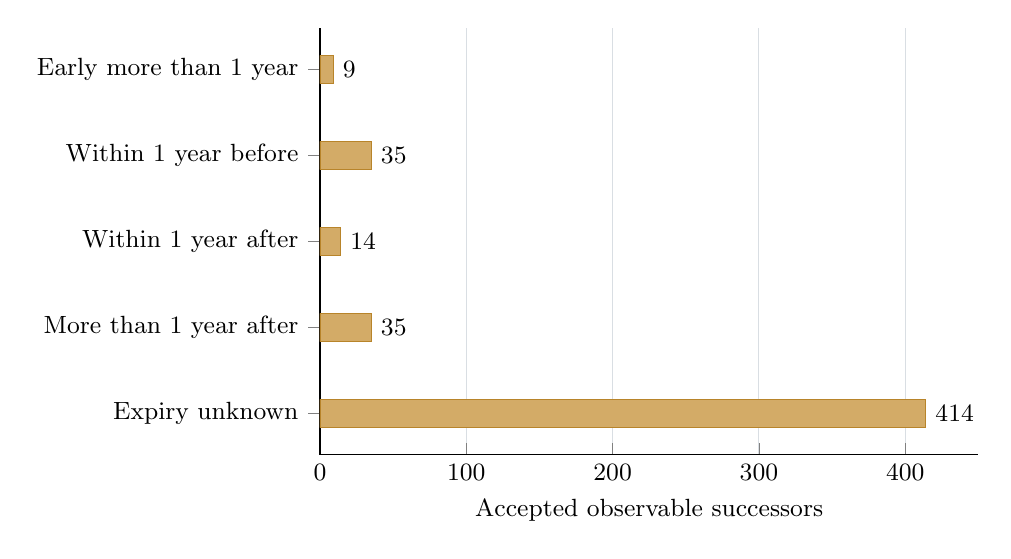
\begin{tikzpicture}
\begin{axis}[
  xbar,width=0.82\textwidth,height=7.0cm,xmin=0,xmax=450,
  symbolic y coords={Early more than 1 year,Within 1 year before,Within 1 year after,More than 1 year after,Expiry unknown},
  ytick=data,y dir=reverse,xlabel={Accepted observable successors},
  axis x line*=bottom,axis y line*=left,xmajorgrids=true,grid style={draw=grid},
  tick label style={font=\small},label style={font=\small},nodes near coords,
  every node near coord/.append style={font=\small,anchor=west},enlarge y limits=0.12
]
\addplot[fill=goldbase!72,draw=goldbase!95!black] coordinates {
  (9,Early more than 1 year) (35,Within 1 year before)
  (14,Within 1 year after) (35,More than 1 year after) (414,Expiry unknown)
};
\end{axis}
\end{tikzpicture}
\caption{Timing classes of the 507 accepted expiry-aware links. Nine very early
links remain because they satisfy both the 0.85 text threshold and positive CPV
continuity.}
\label{fig:timingclasses}
\end{figure}

\subsection{The reviewed benchmark is unchanged}

The benchmark contains 85 evaluable anchors: 22 reviewed positive anchors and 63
reviewed negatives. Table~\ref{tab:benchmark} shows that the expiry-aware policy
makes no rank-one change on this benchmark. Both methods select 10 links: eight are
correct and two choose the wrong successor on positive anchors. Neither method links
a reviewed negative anchor.

\begin{table}[H]
\centering
\caption{Benchmark comparison on all 85 evaluable anchors.}
\label{tab:benchmark}
\begin{tabular}{lrr}
\toprule
\textbf{Metric} & \textbf{V1 text ranking} & \textbf{Expiry-aware} \\
\midrule
Accepted benchmark links & 10 & 10 \\
True positives & 8 & 8 \\
Wrong successor on positive anchor & 2 & 2 \\
False positive on negative anchor & 0 & 0 \\
Precision at rank 1 & 0.8000 & 0.8000 \\
Recall at rank 1 & 0.3636 & 0.3636 \\
Recall at rank 5 & 0.4091 & 0.4091 \\
False-positive rate on negatives & 0.0000 & 0.0000 \\
\bottomrule
\end{tabular}
\end{table}

The locked subset is also unchanged: precision 0.8750, recall 0.4118, and negative
FPR 0.0000 across 69 anchors. These metrics demonstrate non-degradation on the
available review data. They do not demonstrate higher population accuracy because
the benchmark is small, was conditioned on an earlier ranker's top-25 candidates,
and was inspected during method development.

\subsection{Every digital segment retains adequate event volume}

Figure~\ref{fig:segments} compares event counts by primary digital CPV segment. The
largest absolute change occurs in CPV-72 IT services, from 185 to 167 events. Every
segment remains above 30 events, preserving the minimum event volume used by the
project's stratified Kaplan--Meier analysis.

\begin{figure}[H]
\centering
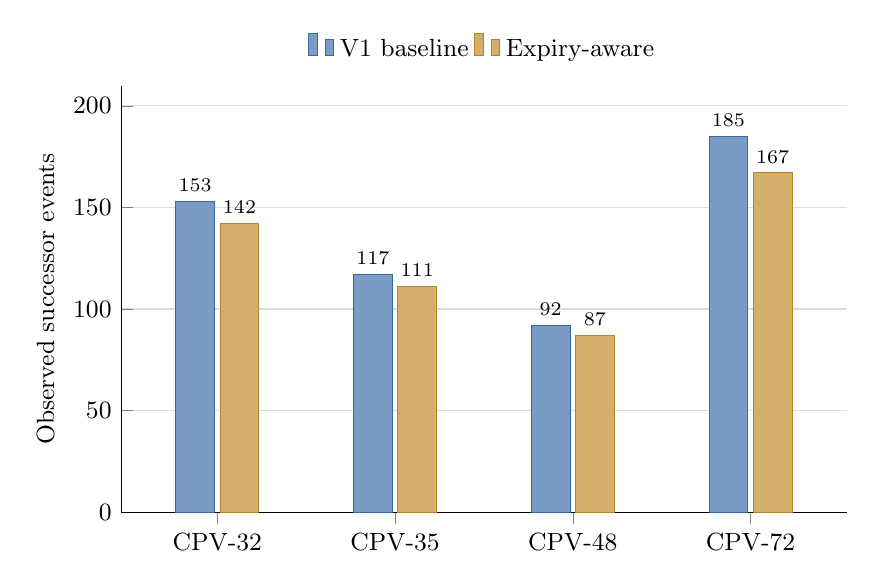
\begin{tikzpicture}
\begin{axis}[
  ybar,width=0.89\textwidth,height=7.0cm,ymin=0,ymax=210,
  symbolic x coords={CPV-32,CPV-35,CPV-48,CPV-72},xtick=data,
  ylabel={Observed successor events},bar width=14pt,enlarge x limits=0.18,
  ymajorgrids=true,grid style={draw=grid},axis x line*=bottom,axis y line*=left,
  tick label style={font=\small},label style={font=\small},
  legend style={at={(0.5,1.03)},anchor=south,legend columns=2,draw=none,font=\small},
  nodes near coords,every node near coord/.append style={font=\scriptsize}
]
\addplot[fill=bluebase!68,draw=bluebase!95!black] coordinates {
  (CPV-32,153) (CPV-35,117) (CPV-48,92) (CPV-72,185)
};
\addplot[fill=goldbase!70,draw=goldbase!95!black] coordinates {
  (CPV-32,142) (CPV-35,111) (CPV-48,87) (CPV-72,167)
};
\legend{V1 baseline,Expiry-aware}
\end{axis}
\end{tikzpicture}
\caption{Observed successor events by digital segment. Counts fall in every segment,
but all remain above the 30-event analysis minimum.}
\label{fig:segments}
\end{figure}

Regional event counts also fall consistently: Bretagne 166 to 152, Normandie 160 to
150, and Pays de la Loire 221 to 205. The change is not isolated to one region.

\section{Survival Dataset and Validation}

For each anchor $a$, the expiry-aware survival row is

\begin{equation}
(\delta_a,T_a)=
\begin{cases}
\left(1,C_{\widehat{y}_a}-A_a\right), & \widehat{y}_a\ne\varnothing,\\
\left(0,C_{\mathrm{cutoff}}-A_a\right), & \widehat{y}_a=\varnothing,
\end{cases}
\end{equation}

where $C_{\mathrm{cutoff}}$ is 31 December 2025. A censored row means no accepted
observable successor before the cutoff; it does not prove that renewal never
occurred.

\begin{table}[H]
\centering
\caption{Structural validation of the expiry-aware survival dataset.}
\label{tab:validation}
\begin{tabular}{lr}
\toprule
\textbf{Check} & \textbf{Result} \\
\midrule
Rows & 3,800 \\
Unique anchor episodes & 3,800 \\
Observed events & 507 \\
Right-censored rows & 3,293 \\
Negative durations & 0 \\
Zero-duration rows & 3 \\
Duplicate anchor episodes & 0 \\
Successor equals anchor & 0 \\
All four segments with at least 30 events & Yes \\
Automated validation passed & Yes \\
\bottomrule
\end{tabular}
\end{table}

The three zero-duration rows are contracts awarded on the observation cutoff with no
accepted successor; they have no follow-up time and are not negative-duration errors.

Documentation-quality diagnostics remain relevant. Among linked anchors, 29.19\%
have a trusted SIREN versus 34.35\% among unlinked anchors. Reliable duration is
present for 18.34\% of linked anchors versus 26.12\% of unlinked anchors. Framework
contracts are more common among linked anchors (24.06\%) than unlinked anchors
(19.13\%). These are descriptive differences, not causal effects.

\section{Promotion Gate, Limitations, and Robustness}

\subsection{The numerical gate passes}

The fixed promotion checks are:

\begin{enumerate}
  \item benchmark precision is at least 0.80;
  \item benchmark false-positive rate on negatives is no higher than v1;
  \item rank-one recall loses no more than one of 22 confirmed positive anchors.
\end{enumerate}

All three checks pass. The recorded recommendation is
\code{review\_then\_consider\_promotion}; manual review remains mandatory.

\subsection{Evidence limitations prevent an automatic claim of superiority}

\begin{itemize}
  \item \textbf{Expiry sparsity.} Expected end is unavailable for 74.9\% of cohort
  contracts and for 414 of 507 accepted links. Those links still use the baseline
  text threshold.
  \item \textbf{Expected end is not always legal expiry.} Only 86 cohort contracts use
  one valid explicit end date. Most resolved dates are calculated from duration and
  either start or award date.
  \item \textbf{The benchmark is small.} Only 22 evaluable positive anchors exist, so
  one outcome changes recall by 4.55 percentage points.
  \item \textbf{The benchmark is ranker-conditioned.} Reviewers saw candidates from a
  previous top-25 export, so buried successors were unavailable for labelling.
  \item \textbf{The locked split is not pristine.} It was inspected during earlier
  development and is evaluation evidence rather than an untouched holdout.
  \item \textbf{Policy thresholds are judgement rules.} The 365-day boundary and
  0.85 early text threshold target an observed failure mode; they were not estimated
  from sufficient labelled data.
  \item \textbf{Successor is not renewal.} A selected pair can represent re-tendering,
  replacement, continuation, or a recurrent need. BOAMP has no legal renewal ID.
\end{itemize}

The evidence supports the claim that the new method is more conservative and better
aligned with contract timing. It does not establish true population precision or
prove that every selected link is a renewal.

\section{Recommended Decision and Next Steps}

The expiry-aware method should remain the preferred promotion candidate and v1 should
remain the reproducible baseline until review is complete. The next work is narrow:

\begin{enumerate}
  \item Review all 42 changed anchors in
  \pathcode{data/processed/boamp_v2/expiry_link_review.csv}.
  \item Assign one label: correct removal, incorrect removal, correct replacement,
  incorrect replacement, or insufficient evidence.
  \item Promote only if review supports the early-evidence gate. If genuine early
  successors are frequently removed, revise the boundary or gate and rerun the same
  parallel evaluation.
  \item If promoted, rerun Kaplan--Meier, Cox, parametric, and watchlist outputs using
  the expiry-aware survival dataset while retaining v1 as sensitivity evidence.
\end{enumerate}

No additional machine-learning model is recommended before this review. The highest
value next labels are the 42 cases where the policy changes the event definition.

\section{Further Questions}

\begin{itemize}
  \item How many of the 40 removed links are genuinely unrelated concurrent procurements?
  \item Do explicit end dates and calculated expected ends have different error rates?
  \item Should candidates more than one year after expected expiry also receive an
  additional functional-continuity gate?
  \item Does the substantive survival conclusion remain stable after a full rerun of
  Kaplan--Meier and regression models on the 507-event dataset?
\end{itemize}

\appendix

\section{Reproducibility and Materialised Artifacts}

\begin{table}[H]
\centering
\caption{Implementation and evidence inventory.}
\small
\begin{tabularx}{\textwidth}{p{4.9cm}X}
\toprule
\textbf{Artifact} & \textbf{Role} \\
\midrule
\pathcode{boamp_pipeline/expiry_linkage.py} & Date resolution, timing classes,
eligibility rule, and deterministic ranking. \\
\pathcode{scripts/evaluate_expiry_aware_linkage.py} & Candidate enrichment,
benchmark comparison, promotion gate, accepted links, and review export. \\
\pathcode{scripts/build_expiry_aware_survival_dataset.py} & Parallel right-censored
survival dataset and validation summary. \\
\pathcode{tests/test_expiry_linkage.py} & Unit tests for date precedence,
boundaries, missingness, gating, and deterministic selection. \\
\pathcode{data/processed/boamp_v2/expiry_aware_linkage_summary.json} & Linkage policy,
benchmark, timing, cohort comparison, and validation metrics. \\
\pathcode{data/processed/boamp_v2/expiry_link_review.csv} & Complete 42-anchor manual
review queue. \\
\pathcode{data/processed/boamp_v2/survival_dataset_expiry_aware.parquet} & Parallel
3,800-row survival dataset with 507 events. \\
\pathcode{data/processed/boamp_v2/survival_dataset_expiry_aware_summary.json} & Survival
validation, segment results, regional results, and linkage-bias diagnostics. \\
\bottomrule
\end{tabularx}
\end{table}

Reproduction commands:

\begin{verbatim}
PYTHONPATH=. python3 scripts/evaluate_expiry_aware_linkage.py --force
PYTHONPATH=. python3 scripts/build_expiry_aware_survival_dataset.py --force
PYTHONPATH=. pytest -q
\end{verbatim}

At report generation, the test suite reports 22 passing tests. The linkage and
survival summary artifacts both report \code{validation\_passed: true}. The v1
candidate pool, linkage outputs, and survival outputs are not overwritten.

\section{Output Schema Additions}

The accepted-link artifact preserves existing candidate fields and adds:

\begin{itemize}
  \item \code{anchor\_expected\_end\_date};
  \item \code{expected\_end\_source};
  \item \code{explicit\_start\_date} and \code{explicit\_end\_date};
  \item \code{explicit\_start\_date\_count} and \code{explicit\_end\_date\_count};
  \item \code{days\_from\_expected\_end};
  \item \code{timing\_class};
  \item \code{selection\_method};
  \item \code{expiry\_linkage\_version}.
\end{itemize}

The parallel survival artifact carries timing and selection fields for linked events
while retaining the existing cohort grain and censoring definition.

\end{document}
